\documentclass{article}

\usepackage[ngerman]{babel}										% Statt german, \autoref zeigt damit "Abbildung x" an
\usepackage{graphicx}											% Graphiken einbinden
\usepackage[left=3cm,right=3cm,top=3cm,bottom=3cm]{geometry}	% Abstände zu den Papierrändern
\usepackage[utf8]{inputenc}										% Zeichenkodierung
\usepackage{mathtools}											% Stellt Mathe-Umgebung bereit
\usepackage{float}												% Improves floating elements
\usepackage{lmodern}											% Andere Schriftart (bessere Druckbarkeit)
\usepackage{pdfpages}											% Einbinden von PDF-Dokumenten
\usepackage{fancyhdr}											% Fancy Headers / Footers
\usepackage{listliketab}										% Lists with tab stops
\usepackage{setspace}											% Anpassung von Zeilenabständen
\usepackage{siunitx}											% Korrekte Darstellungen von Einheiten (\SI{1.5}{\milli\volt})
\usepackage{hyperref}   										% Objekte referenzieren (\autoref)
\usepackage{subcaption}
\usepackage{listings}
\DeclareSIUnit{\Bit}{Bit} % bits 

% dark mode
%\usepackage{xcolor}			
%\pagecolor[rgb]{0,0,0}
%\color[rgb]{1,1,1}

\setlength{\parindent}{0em}										% Keine Einrückung bei Absatzbeginn
\setlength{\parskip}{1em}										% Dafür vert. Abstand zw. Absätzen

\renewcommand{\arraystretch}{1.2}								% Verzeichnisse kompakter darstellen

\newcommand{\tbf}{\textbf}										% Shortcut für fetten Text

\makeatletter
\g@addto@macro\bfseries{\boldmath}								% \mathbf nicht im Inhaltsverzeichnis darstellen
\makeatother

\pagestyle{fancy}												% Benutzung von fancyhdr
\sisetup{
	locale = DE,
	per-mode=fraction,
	fraction-function=\tfrac
	}

\lhead{}
\rhead{}

% anpassen!
\chead{Regelungstechnik - Praktikum 1}
\lfoot{08.05.2020}
\cfoot{Felix Arndt, Loïc Fernau, Niklas Bammann}

\rfoot{Seite \thepage}

\usepackage{titlesec}
\titlespacing\section{0pt}{12pt plus 4pt minus 2pt}{0pt plus 2pt minus 2pt}
\titlespacing\subsection{0pt}{0pt}{0pt}
\titlespacing\subsubsection{0pt}{12pt plus 4pt minus 2pt}{0pt plus 2pt minus 2pt}


\begin{document}
	% Titelseite anpassen
	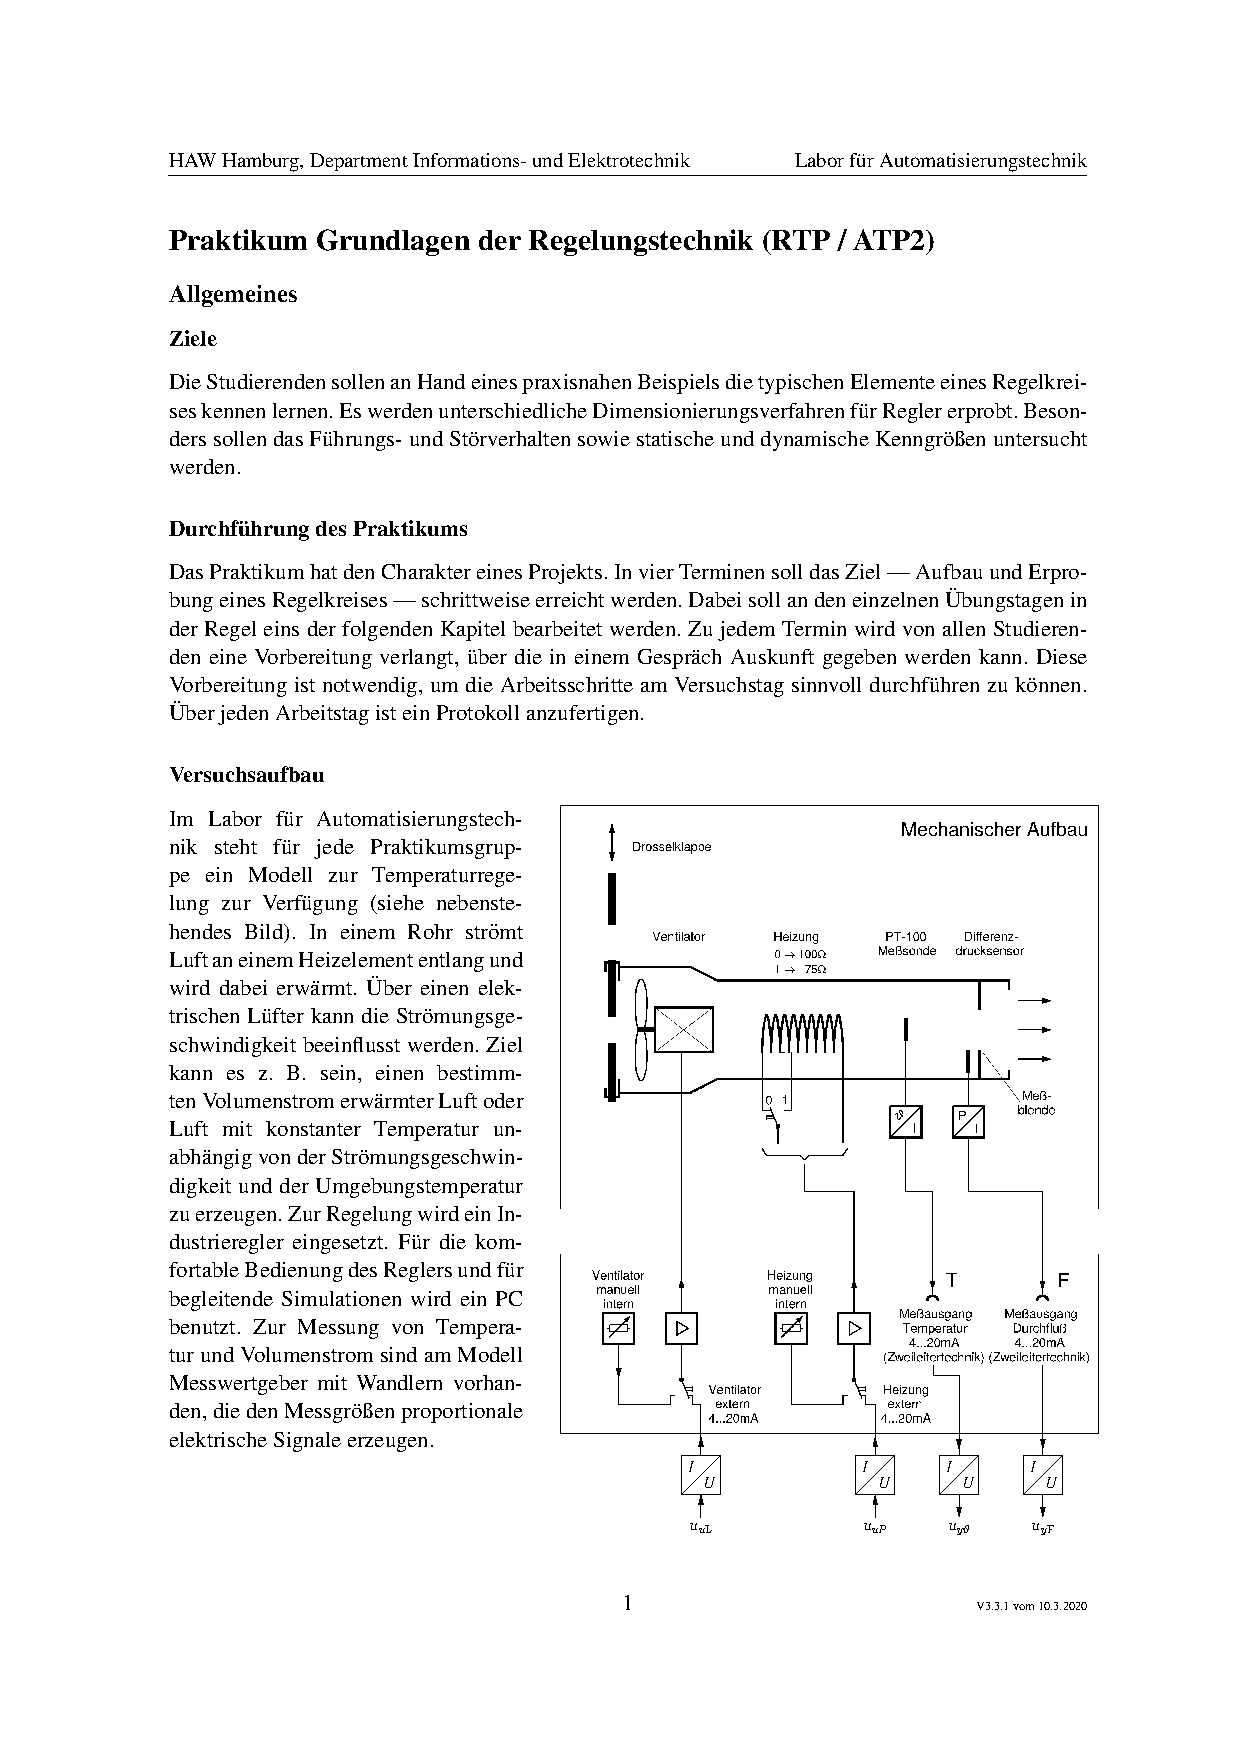
\includepdf[pages={1-6}]{pdf_ext/200310_Anleitung_RTP_V3_3_1.pdf}

 	\begin{titlepage}
 		\begin{flushright}
			
\includegraphics[width=0.5\textwidth]{img/title.png}\\[2cm]
		\end{flushright}
		
		\begin{center}
			%\textsc{\LARGE Hochschule für angewandte Wissenschaften}\\[0.2cm]
			%\textsc{\LARGE Hamburg}\\[1.5cm]
			\textsc{\Large Regelungstechnik}
			\rule{\linewidth}{0.5mm}\\[1.5cm]
			{ \huge \bfseries Praktikumsprotokoll}
			\rule{\linewidth}{0.5mm}\\[2cm]
			% Termin anpassen
			{ \huge \bfseries Die Temperatur-Regelstrecke}\\[2cm]
            
            \LARGE Felix Arndt \\
			\LARGE Loïc Fernau \\
			\LARGE Niklas Bammann \\[4cm]
			% Gruppe anpassen
			\large RTP1
		\end{center}
	\end{titlepage}
	\newpage
	
	\renewcommand{\baselinestretch}{0.8}\normalsize
	\tableofcontents
	\listoffigures
	\listoftables
	\renewcommand{\baselinestretch}{1.0}\normalsize
	
	\newpage

	\setlength{\headsep}{0.4em}
	

	\section{Einleitung}

Im diesem Versuch sollen die Eigenschaften einer Regelstrecke untersucht werden. Die Regelstrecke besteht aus einem Lüfter, einer Heizung, einem Temperatur- und einem Drucksensor. Für diesen Versuch sind zunächst die Auswirkungen von Lüfterdrehzahl- und Heizleistungsänderungen auf die Lufttemperatur am Ausgang interessant. Es werden sowohl Messungen im stationären Zustand als auch mit dynamischen Eingangsignalen gemacht. Ziel der Messungen ist es, ein akkurates mathematisches Modell der Regelstrecke zu erstellen. Dafür werden Sprungantworten aufgezeichnet und anschließend numerisch an ein entsprechendes Modell gefittet.

%\subsection{Verwendete Geräte/Software}

%Für den Versuch wird folgende Geräte/Software verwendet:

%\begin{table}[ht]
%    \centering
%    \begin{tabular}{|c|c|c|c|}\hline
%    \tbf{Gerätetyp}     & \tbf{Bezeichnung} \\ \hline
%                        &                   \\ \hline
%                        &                   \\ \hline
%    \end{tabular}
%    \caption{Auflistung der Geräte/Software}
%\end{table}

	\section{Vorbereitung}

\subsection{Aufgabe V1.1}

% Rekapitulieren Sie die Begriffe Kennlinienfeld, Arbeitspunkt und stationäres Verhalten. Welche Gleichung im Grundlagenteil beschreibt die zu messenden Kennlinienfelder und welche (mathematischen) Abhängigkeiten erwarten Sie für uyϑ = f(uuP ) bzw. uyϑ = f(uuL)?

\subsubsection{Kennlinienfeld}

Ein Kennlinienfeld ist eine Darstellung von mehreren Kennlinien von einem System im gleichen Diagramm, die sich um einen Parameter unterscheiden.

\subsubsection{Arbeitspunkt}

Der Arbeitspunkt ist ein Punkt auf der Kennlinie, an dem der Zustand eines Systems im Betrieb gehalten wird.

\subsubsection{Stationäres Verhalten}

Ein System zeigt sein stationäres Verhalten, wenn äußere Einflüsse sich nicht verändern und das System eingeschwungen ist.

\subsubsection{Gleichung der Kennlinienfelder}

Die für uns interessanten Kennlinien beschreiben den Temperaturanstieg in Abhängigkeit von der zugeführten Leistung. Weitere Parameter sind die die Dichte und spezifische Wärmekapazität der Luft, sowie die Strömungsgeschwindigkeit. 

\[ \Delta\vartheta  = \frac{1}{c_L \varrho_L A}\frac{1}{v}P_{th} \]

Durch erhöhen der Strömungsgeschwindigkeit wird die Temperatur abfallen, da die zugeführte Energie auf mehr Luftmasse aufgeteilt wird. Durch erhöhen der Heizleistung erhöht sich die Temperatur, da die Luft eine höhere Energiemenge aufnehmen muss.

\subsection{Aufgabe V1.2}

% Berechnen Sie mit Hilfe der Übertragungsfunktion einen analytischen Ausdruck für die Sprungantwort des Temperaturverlaufs bei einem Heizleistungssprung Pel(t) = Pˆelσ(t).

\[ G_{S}(s) = \frac{\vartheta(s)}{P_{el}(s)} = K_{S} \frac{e^{-T_{t}s}}{1 + T_{S}s} \]
\[ \]


\[ \vartheta\left(t\right) = \hat{P}_{el} \cdot K_s \cdot \left(1-e^{-\frac{1}{T_s}\cdot\left(t-T_t\right) }\right) \]

\subsection{Aufgabe V1.3 und Aufgabe V1.4}

% Simulieren und plotten Sie den Zeitverlauf der Sprungantwort mit Matlab/Simulink für Pel(t) = 10 W · σ(t).

% Rekapitulieren Sie aus dem Grundlagenteil den Einfluss (mathematische Abhängigkeit) der Heizleistung auf die Streckenparameter. Plotten oder skizzieren Sie hierzu die Sprungantworten für a) Pel(t) = 10 W · σ(t), b) Pel(t) = 20 W · σ(t), c) Pel(t) = 30 W · σ(t). und überlegen Sie sich eine physikalische Interpretation.

In \autoref{fig:V1_4_kennlinienfeld} wird das Kennlinienfeld für \( P_{el} = \SI{10}{\watt}\), \(\SI{20}{\watt}\) und \(\SI{30}{\watt}\) gezeigt. Es ist deutlich zu erkennen, dass eine höhere zugeführte Leistung mit einer höheren Temperaturänderung einhergeht. Das liegt daran, dass eine höhere Leistung dem System im gleichen Zeitraum eine größere thermische Energiemenge zuführt. Dadurch muss auch die Temperatur stärker ansteigen.

\begin{figure}[H]
    \begin{center}
        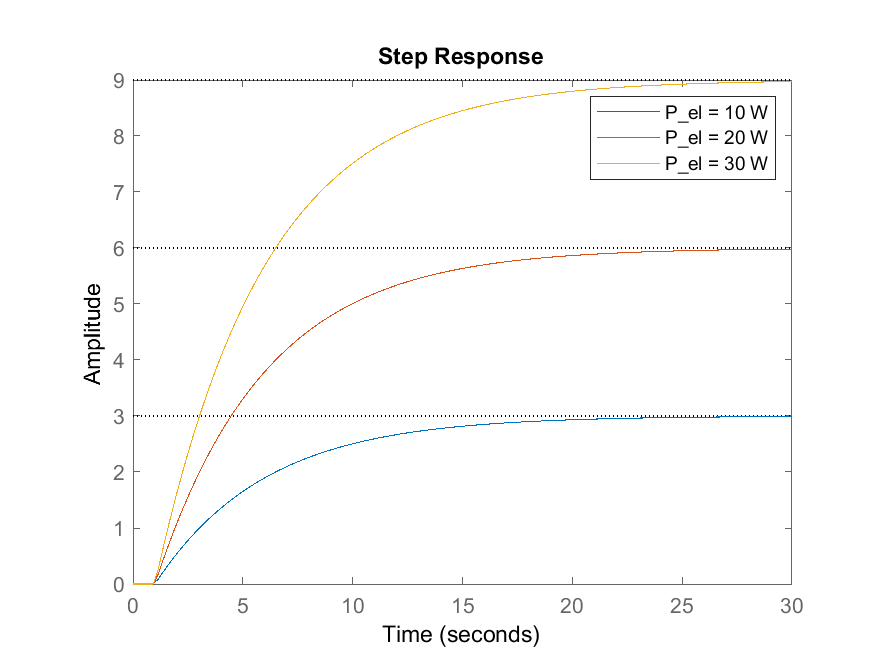
\includegraphics[width=0.8\textwidth]{img/V1_4.png}
        \caption{Kennliniefeld für \( P_{el} = \SI{10}{\watt}\), \(\SI{20}{\watt}\) und \(\SI{30}{\watt}\)}
        \label{fig:V1_4_kennlinienfeld}
    \end{center}
\end{figure}

\newpage

\subsection{Aufgabe V1.5}

% Wiederholen Sie V1.4 mit dem Einfluss der Lüftergeschwindigkeit und überlegen Sie sich, was passiert, wenn man die Lüftergeschwindigkeit halbiert bzw. verdoppelt. Plotten oder skizzieren Sie hierzu die Temperaturverläufe für Pel(t) = 10 W · σ(t) unter der Annahme der folgenden Strömungsgeschwindigkeiten: a) v = vL, b) v = vL 2 , c) v = 2 · vL.

In \autoref{fig:V1_5_kennlinienfeld} wird das Kennlinienfeld für \( v = v_L\), \(\frac{v_L}{2}\) und \(2\cdot v_L\) gezeigt. Die erreichte Temperaturänderung halbiert sich bei doppelter Strömungsgeschwindigkeit und verdoppelt sich bei halbierung der Strömungsgeschwindigkeit. Das liegt daran, dass sich die dem System zugeführte Energie im gleichen Zeitraum auf die halbe bzw. doppelte Menge Luft kommt.

\begin{figure}[H]
    \begin{center}
        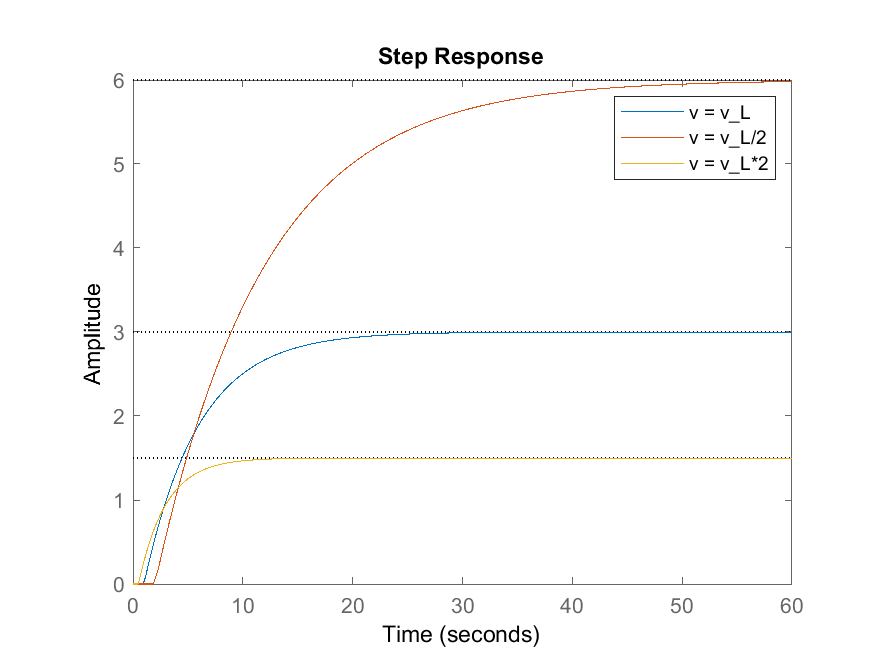
\includegraphics[width=0.8\textwidth]{img/V1_5.png}
        \caption{Kennliniefeld für \( v = v_L\), \(\frac{v_L}{2}\) und \(2\cdot v_L\)}
        \label{fig:V1_5_kennlinienfeld}
    \end{center}
\end{figure}

\newpage
	\section{Messungen}

Der erste Teil der Messungen untersucht stationäre Betriebsszustände, der zweite Teil untersucht das dynamische Verhalten der Strecke.

\subsection{Stationärer Zustand am Arbeitspunkt}
%Messen Sie mit einem elektronischen Temperaturfühler die Temperatur des Luftstroms am Arbeitspunkt in ◦C und notieren Sie die zugehörigen Werte der Messwertgeber (uyϑ0 , uyF0 ),nachdem sich der stationäare Zustand eingestellt hat.

%Wiederholen Sie die Messungen für 40%, 50% und 60% Heizleistung indem Sie für jede Heizleistung die LÜfterspannung auf 60%, 50% und 40% variieren.

Gemessen wurde die Ausgangsspannung des Temperatur- und des Luftstromsensors bei variierten Stellgraden für Heiz- und Lüfterleistung. Hierbei wurden die neun möglichen Kombination der Werte \(\SI{40}{\percent}\), \( \SI{50}{\percent}\) und \(\SI{60}{\percent}\) untersucht. Vor dem Ablesen der Werte wurde gewartet, bis diese sich stabilisieren. Die Messwerte sind in \autoref{tab:M1_12_werte} eingetragen.

\begin{table}[ht]
    \centering
    \begin{tabular}{|c|c|c|c|c|}\hline
    \tbf{Heizung}     & \tbf{Lüfter}  & \tbf{Temperatur}   & \tbf{Luftstrom}     & \tbf{Temperatur } \\ \hline
    \(u_{uP}\)                 & \(u_{uL}\)                & \(u_{y\vartheta}\)        & \(u_{yF}\)                & \(\vartheta\) \\ \hline
    \SI{4}{\volt}               & \SI{4}{\volt}             & \SI{3.7}{\volt}           & \SI{2.51}{\volt}          & \SI{41.3}{\celsius} \\ \hline
    \SI{5}{\volt}               & \SI{4}{\volt}             & \SI{4.37}{\volt}          & \SI{2.48}{\volt}          & \SI{44.4}{\celsius} \\ \hline
    \SI{6}{\volt}               & \SI{4}{\volt}             & \SI{4.97}{\volt}          & \SI{2.49}{\volt}          & \SI{47.2}{\celsius} \\ \hline
    \SI{4}{\volt}               & \SI{5}{\volt}             & \SI{3.23}{\volt}          & \SI{3.59}{\volt}          & \SI{39.1}{\celsius} \\ \hline
    \SI{5}{\volt}               & \SI{5}{\volt}             & \SI{3.76}{\volt}          & \SI{3.38}{\volt}          & \SI{41.7}{\celsius} \\ \hline
    \SI{6}{\volt}               & \SI{5}{\volt}             & \SI{4.34}{\volt}          & \SI{3.4}{\volt}           & \SI{44.3}{\celsius} \\ \hline
    \SI{4}{\volt}               & \SI{6}{\volt}             & \SI{3.06}{\volt}          & \SI{4.23}{\volt}          & \SI{38.4}{\celsius} \\ \hline
    \SI{5}{\volt}               & \SI{6}{\volt}             & \SI{3.48}{\volt}          & \SI{4.45}{\volt}          & \SI{40.3}{\celsius} \\ \hline
    \SI{6}{\volt}               & \SI{6}{\volt}             & \SI{3.96}{\volt}          & \SI{4.25}{\volt}          & \SI{42.6}{\celsius} \\ \hline
    \end{tabular}
    \caption{Sollwertkombinationen und resultierende Messwerte}
    \label{tab:M1_12_werte}
\end{table}


\subsection{Sprungantworten für Eingangssprünge der Heizleistung}

% Bei den nachfolgenden Oszillogrammen ist auf eine hohe Auflösung zu achten (größtmögliche Darstellung der Kurven). Um den kleinstmöglichen Messbereich am Oszilloskop wählen zu können, ist der Offset des aufzuzeichnenden Signales mit einer in Serie geschalteten externen Spannungsquelle zu kompensieren.

% Zeichnen Sie die Sprungantworten der Temperatur für Eingangssprünge der Heizleistung von 40% auf 60% und von 60% auf 40% auf.

% lüfter 5v
% auf 60 bzw 40 % einstellen
Für die Messung des dynamischen Verhaltens wird zunächst die Lüfterleistung auf \( \SI{50}{\percent} \) eingestellt. Anschließend wird die Heizleistung auf \( \SI{60}{\percent} \) eingestellt und gewartet, bis sich die Werte stabilisieren. Mithilfe eines externen Netzteil wird ein Offset auf die Ausgangsspannung des Temperatursensors gelegt, um die absolute Ausgangspannung zu reduzieren. Dadurch kann ein kleinerer Messbereich des Oszilloskops verwendet werden, was zu einer deutlichen Verbesserung der Auflösung führt.

In \autoref{fig:M1_3_a_step} und \autoref{fig:M1_3_a_step} sind die Sollwertsprünge und Sprungantworte der Regelstrecken abgebildet.

\newpage

\begin{figure}[H]
    \begin{center}
        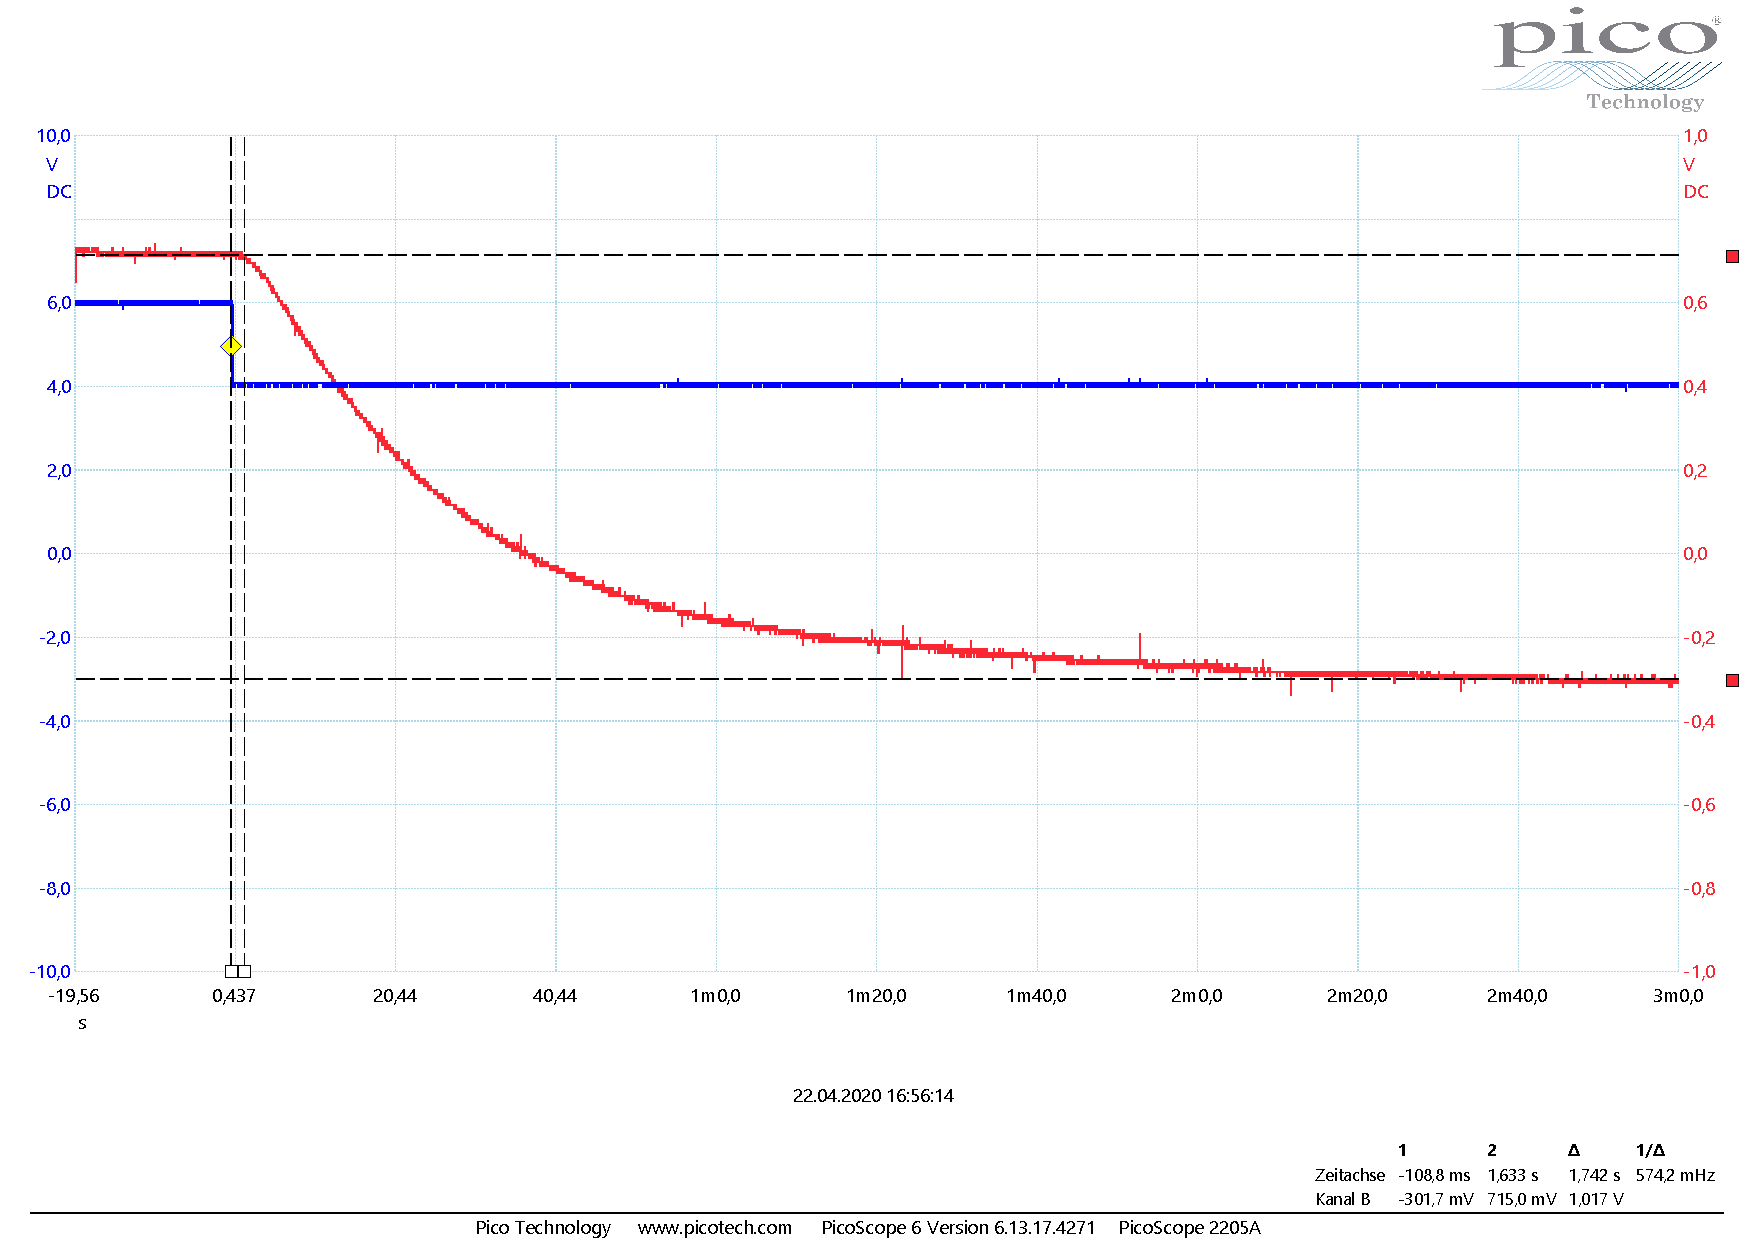
\includegraphics[width=0.85\textwidth]{pdf_ext/anlage5_messung1_u_uP_60_40.pdf}
        \caption{Sprungantwort bei Sollwertsprung von \( \SI{60}{\percent} \) auf \( \SI{40}{\percent} \)}
        \label{fig:M1_3_a_step}
    \end{center}
\end{figure}

\begin{figure}[H]
    \begin{center}
        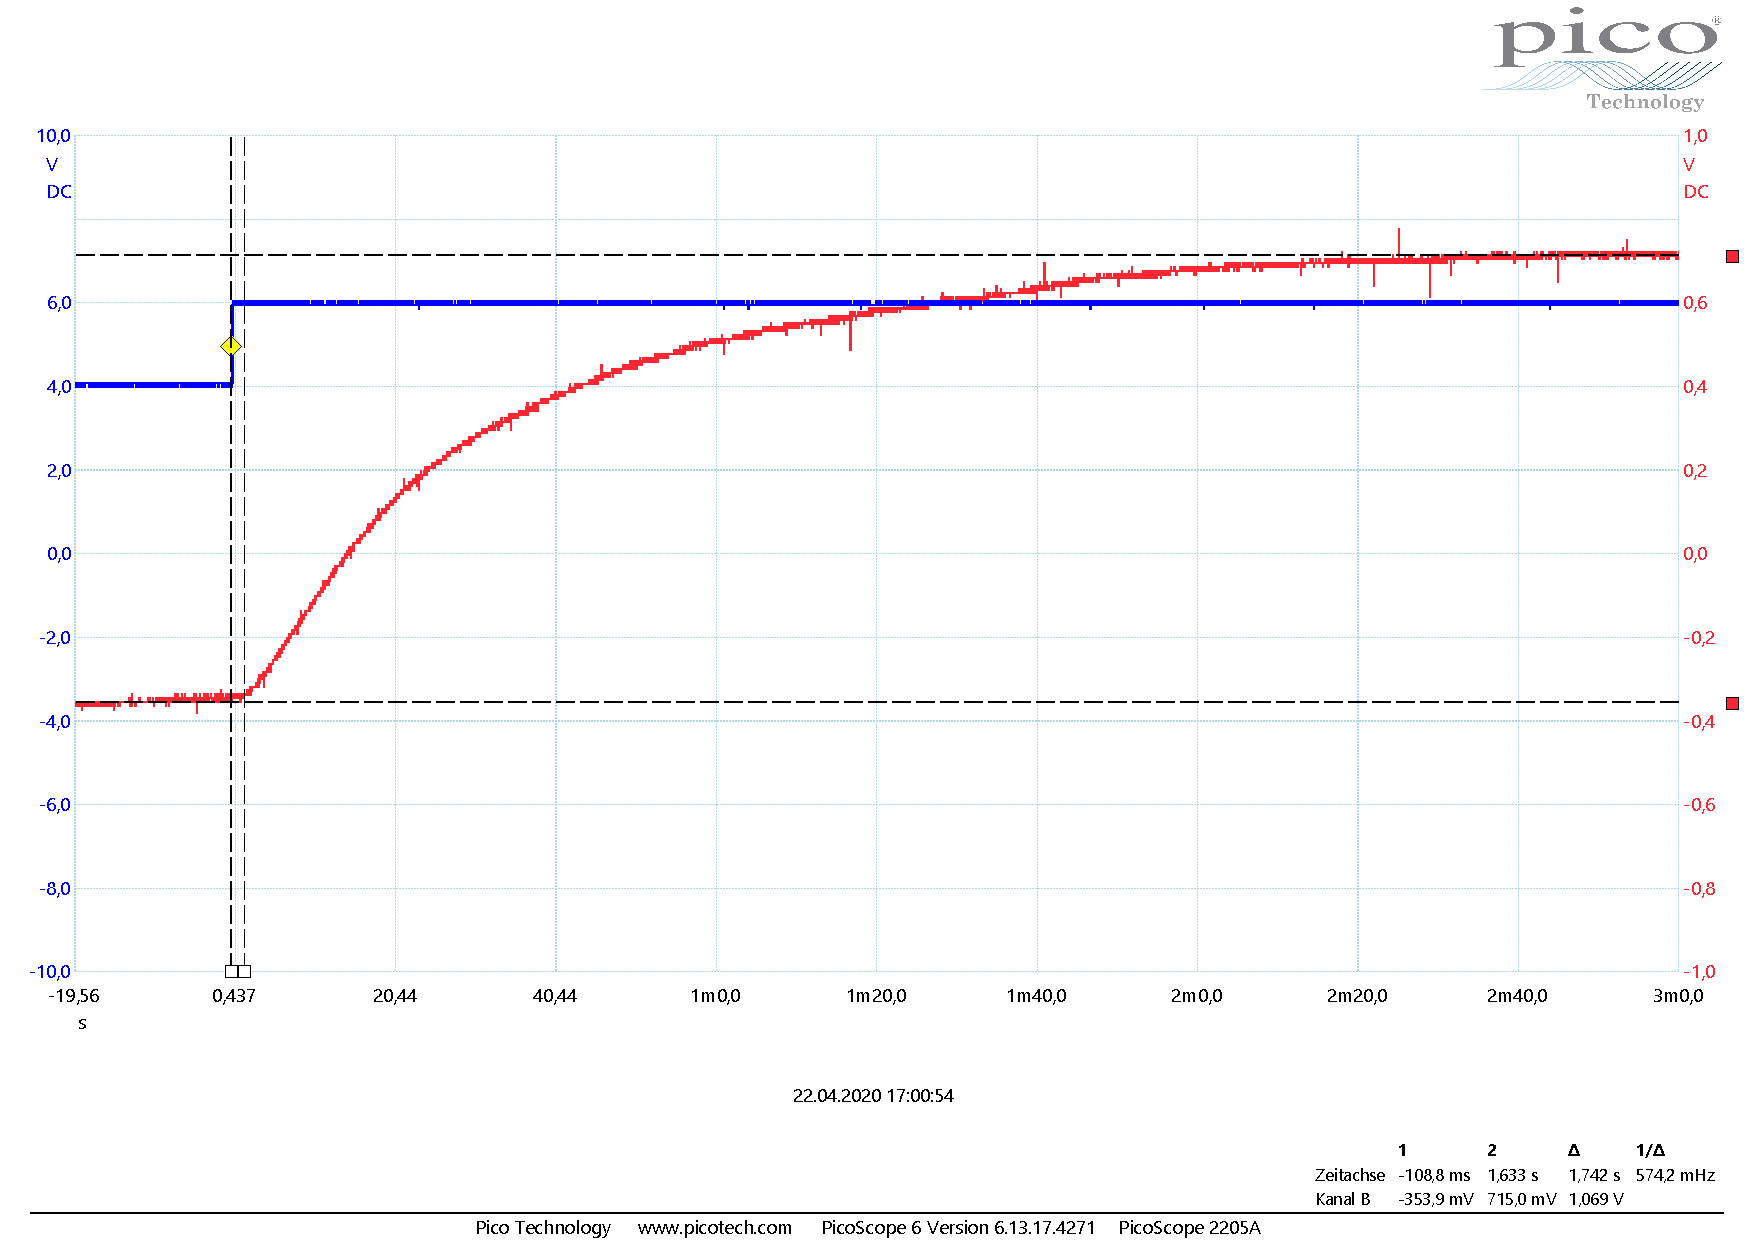
\includegraphics[width=0.85\textwidth]{pdf_ext/anlage5_messung2_u_uP_40_60.pdf}
        \caption{Sprungantwort bei Sollwertsprung von \( \SI{40}{\percent} \) auf \( \SI{60}{\percent} \)}
        \label{fig:M1_3_b_step}
    \end{center}
\end{figure}
 
 \newpage
 
	\section{Auswertung}

\subsection{Stationäres Verhalten}

Um die Kennlinienfelder zu erstellen werden die Messwerte aus \autoref{tab:M1_12_werte} in Matlab übernommen und als Punkte geplottet. Anschließend wird für jeden Parameterwert eine Ausgleichsgerade geplotttet. Davon ausgehend, dass die Heiz- und Lüfterleistung proportional zum jeweiligen Sollwert sind, kann mit diesen Kennlinienfelder eine Aussage getroffen werden, auf welche Temperatur sich die Regelstrecke bei bestimmten einstellt.

Das Kennlinienfeld für variablen Heizungssollwert und konstanten Lüftersollwert als Parameter ist in \autoref{fig:A1_1_kennlinienfeld} abgebildet. Das Kennlinienfeld für variablen Lüftersollwert und konstanten Heizungssollwert als Parameter ist in \autoref{fig:A1_2_kennlinienfeld} abgebildet.

\begin{figure}[h]
    \begin{center}
        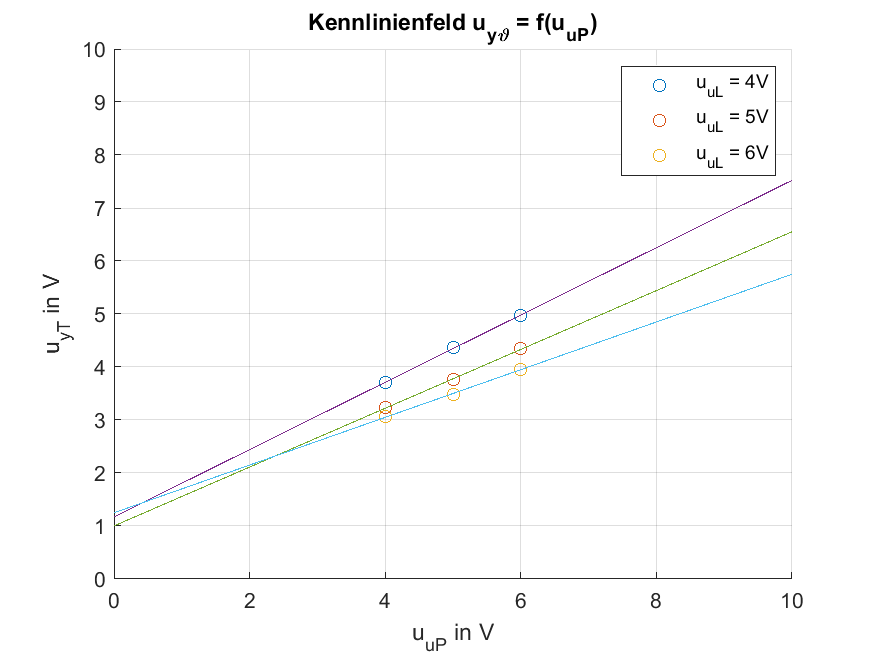
\includegraphics[width=0.8\textwidth]{img/A1_1.png}
        \caption{Kennlinienfeld \( U_{y\vartheta} = f\left(U_{uP}\right) \)}
        \label{fig:A1_1_kennlinienfeld}
    \end{center}
\end{figure}

\newpage

\begin{figure}[h]
    \begin{center}
        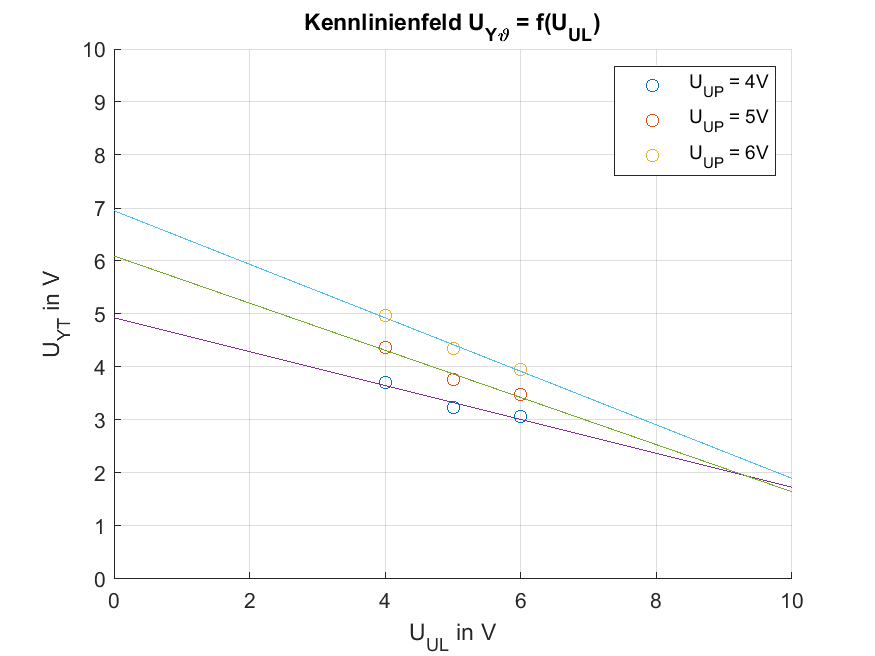
\includegraphics[width=0.8\textwidth]{img/A1_2.png}
        \caption{Kennlinienfeld \( U_{y\vartheta} = f\left(U_{uL}\right) \)}
        \label{fig:A1_2_kennlinienfeld}
    \end{center}
\end{figure}

\subsubsection{A1.4: Lineare Interpolation}

Verwendet man für die Ausgleichsgerade die etwas ungenauere Formel \( y = m\cdot x \), erhält man aus der numerischen Berechnung den Parameter  \( m = \SI{0.7501}{} \), Dies ist dementsprechend die Streckenverstärkung:

\[K_{ges} = \frac{\Delta u_{y\theta}}{\Delta u_{uP}} = K_u \cdot K_S \cdot K_M = \SI{0.7501}{} \]

Weiterhin gilt:

\[K_S = \frac{\Delta \theta}{\Delta P_{el}} ; K_u = \frac{\Delta P_{el}}{\Delta u_{uP}} ; K_M = \frac{\Delta u_{y\theta}}{\Delta \theta}\]


Um die Werte für \( U_{y\vartheta} \) und \( U_{uP} \) bei der gegeben Temperatur \( \vartheta = \SI{46}{\celsius} \) auszurechnen, wird zunächst die Steigung einer Ausgleichsgerade für das Verhältnis zwischen Temperatur und Ausgangsspannung des Temperatursensors numerisch berechnet. Anschließend lassen sich die Spannungswerte berechnen:

\[ U_{y\vartheta} = f\left(\vartheta\right) = \frac{\vartheta}{\SI{10.9512}{\celsius\per\volt}} = \frac{\SI{46}{\celsius}}{\SI{10.9512}{\celsius\per\volt}} = \SI{4,2}{\volt} \]
\[ U_{uP} = \frac{U_{y\vartheta}}{K_S} = \frac{\SI{4,2}{\volt}}{\SI{0.7501}{}} = \SI{5,599}{\volt} \]

\newpage


\subsection{Dynamisches Verhalten}

Um das dynamische Verhalten der Regelstrecke abzubilden, soll als Modell ein PT1-Glied mit Totzeit verwendet werden.  Das Modell lässt sich durch folgende Formel beschreiben:

\[ G_S\left(s\right) = \frac{\vartheta\left(s\right)}{P_{el}\left(s\right)} = K_S \frac{e^{-T_t s}}{1+T_S s}\]

Um die Parameter zu bestimmen, werden die Messwert zunächst in Matlab geladen und der Zeitindex des Sprungs manuell bestimmt. Anschließend wird der Mittelwert des Heizungs-Stellgrades jeweils vor und nach dem Sprung bestimmt. Der Mittelwert vor dem Sprung wird elementweise von dem gesamten Datensatz abgezogen, um den Offset auf null zu setzen. Der Mittelwert nach dem Sprung wird für die Berechnung der Proportionalverstärkung des System benötigt. Vom dem Temperatur-Istwert werden ebenfalls alle Werte vor dem Sprung gemittelt und elementweise von dem Istwert-Datensatz abgezogen, ebenfalls um den Offset zu entfernen. Anschließend werden die Werte der letzten 10 Sekunden gemittelt und als Endwert angenommen. Mit dem Endwert und die mittleren Sollwert nach dem Sprung wird die Proportionalverstärkung berechnet. Anschließend wird mit diesem Wert ein das mathematische Modell der Regelstrecke gebildet. Die Parameter für die Ausgleichs- und Verzugszeit werden anschließend nur Anwendung der Methode der kleinsten Quadrate ermittelt. Dafür werden Werte in einem relativ weiten Bereich durchprobiert. Das Modell wird mit dem gemessenen Heizungs-Sollwert simuliert und anschließend die Differenz zur gemessenen Sprungantwort berechnet und ausgewertet. Die optimalen Parameter werden ausgegeben und sind in \autoref{tab:A1_6_parameter} gelistet. Die aufbereiteten Daten und die Sprungantwort des Modells sind in \autoref{fig:A1_6_a_fit} und \autoref{fig:A1_6_a_fit} als Plot dargestellt.

\begin{figure}[h]
    \begin{center}
        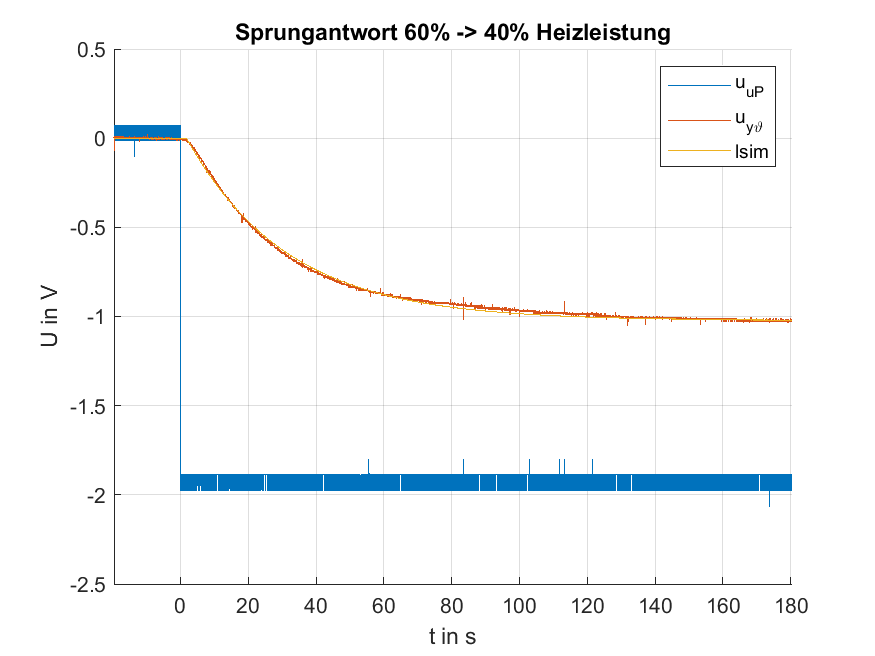
\includegraphics[width=0.8\textwidth]{img/A1_6_a.png}
        \caption{Plot der gemessen Werte und optimalem Modell für Messung 1}
        \label{fig:A1_6_a_fit}
    \end{center}
\end{figure}

\begin{figure}[h]
    \begin{center}
        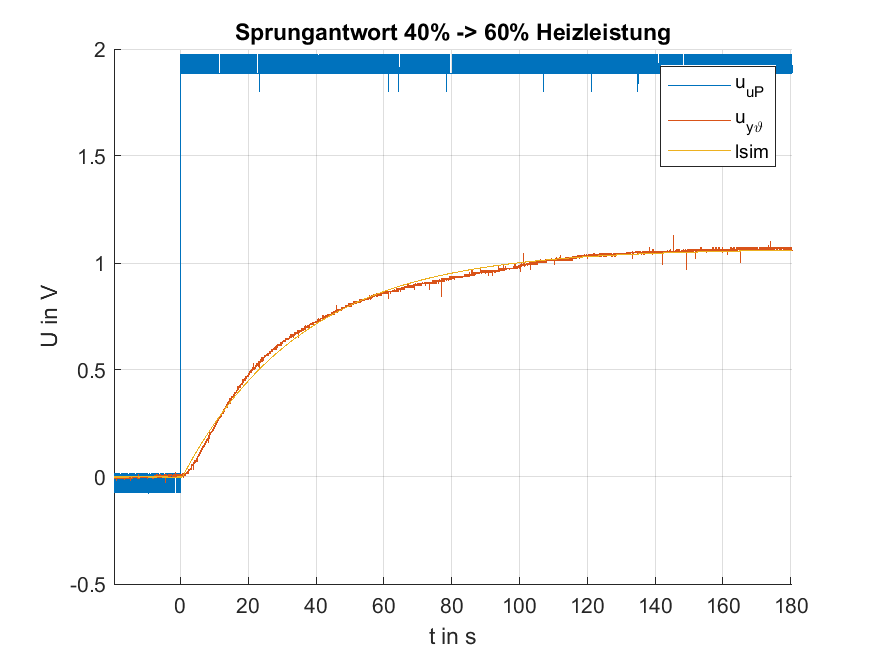
\includegraphics[width=0.8\textwidth]{img/A1_6_b.png}
        \caption{Plot der gemessen Werte und optimalem Modell für Messung 2}
        \label{fig:A1_6_a_fit}
    \end{center}
\end{figure}



\begin{table}[H]
    \begin{center}
    \begin{tabular}{|c|c|c|c|}\hline
    \tbf{Parameter} & \tbf{Messung 1}               & \tbf{Messung 2}               \\ \hline
    \( K_s \)       & \SI{0.5378}{\kelvin\per\watt} & \SI{0.5611}{\kelvin\per\watt} \\ \hline
    \( T_s \)       & \SI{29.77}{\second}           & \SI{35.52}{\second}           \\ \hline
    \( T_t \)       & \SI{1.83}{\second}            & \SI{0.58}{\second}            \\ \hline
    \end{tabular}
    \caption{Per numerischer Berechnung bestimmte optimale Parameter}
    \label{tab:A1_6_parameter}
    \end{center}
\end{table}
	
\section{TESTEst1234}

	


	\newpage



\end{document}